\qns{Polynomial Multiplication and Discrete-Time Convolution [Adapted from EE 120]}
% Adapted and extended by Ken Zheng for EECS 16A Fall 2025 Discussion

The impulse response of a real, discrete-time FIR filter $\mathsf{A}$ is described by  
$$a[n]=a_0 \delta[n]+a_1 \delta[n-1]+\cdots + a_N \delta[n-N], \quad \text{where } N\in \{1,2,3,\ldots\}.$$

\begin{enumerate}[(a)]
\item Show that the frequency response $A(\omega)$ of the filter is a polynomial, in terms of $e^{-i\omega}$, whose coefficients have a simple relationship with the impulse response values $a_0,\ldots,a_N$.

\ans{

    Substituting \(a[n]\) into the frequency response formula we see that:
    \begin{equation*}
        A(w) = \sum_{n=-\infty}^{\infty} a[n]e^{-iwn}
    \end{equation*}
    As $a[n] = 0$ outside the range of $n = 0$ to $n = N$ ,
    \begin{equation*}
        A(w) = a_0 e^{-iw\cdot 0} + a_1 e^{-iw\cdot 1} + \ldots + a_N e^{-iw\cdot N}
    \end{equation*}
    \begin{equation*}
        = a_0 + a_1 e^{-iw} + \ldots + a_N e^{-iwN}
    \end{equation*}
}
\item Suppose the filter $\mathsf{A}$ is placed in a cascade (series) interconnection with another discrete-time FIR filter $\mathsf{B}$ whose impulse response is described by  
$$b[n]=b_0 \delta[n]+b_1 \delta[n-1]+\cdots + b_M \delta[n-M],\quad \text{where } M\in \{1,2,3,\ldots\}.$$

The cascade structure, which we call $\mathsf{C}$, is shown in the figure below.
\vspace{4pt}

\centerline{
    \begin{Described}{Block diagram: input x enters block A, whose output feeds block B, and block B's output is y. An outer box enclosing both blocks is labelled C.}
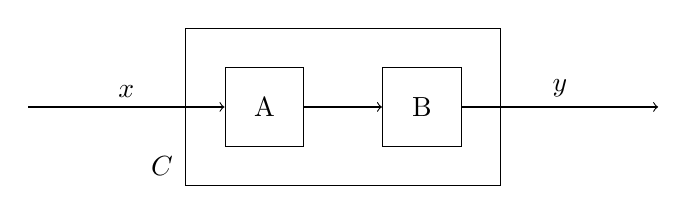
\begin{tikzpicture}
        % Define nodes for blocks A and B
        \node[draw, rectangle, minimum width=1cm, minimum height=1cm] (A) at (0,0) {A};
        \node[draw, rectangle, minimum width=1cm, minimum height=1cm] (B) at (2,0) {B};
        
        % Draw the outer rectangle
        \draw (-1, 1) rectangle (3, -1);
        
        % Draw arrows and labels
        \draw[->] (-3, 0) -- (A.west) node[midway,above] {$x$};
        \draw[->] (A.east) -- (B.west);
        \draw[->] (B.east) -- (5, 0) node[midway,above] {$y$};
        
        % Label C 
        \node at (-1.3, -0.5) [below] {$C$};
    \end{tikzpicture}
\end{Described}
}
Let $c$ denote the impulse response of the cascade interconnection.

\begin{enumerate}[(i)]
\item Express $c$ in terms of $a$ and $b$.
    
\ans{

        The impulse response \(c\) of the cascade interconnection is given by 
        \begin{equation*}
            c[n] = (a * b)[n] = \sum_{k=-\infty}^{\infty} a[k]\,b[n-k]
        \end{equation*}
         Substituting \(n = 0\):
        \begin{equation*}
            c_0 = a_0 b_0
        \end{equation*}
        \(n = 1\):
        \begin{equation*}
            c_1 = a_0 b_1 + a_1 b_0 
        \end{equation*}
        \(n = 2\):
        \begin{equation*}
            c_2 = a_0 b_2 + a_1 b_1 + a_2 b_0
        \end{equation*}
        And so on...
    
        Thus, we can write:
        \begin{equation*}
            c_n = \sum_{k=\max(0,n-M)}^{\min(n, N)} a_k b_{n-k}
        \end{equation*}
        \null\hfill for \(n = 0, 1, \ldots, N + M\)
        
        where we found the bounds of summation from the two conditions that ensure we are indexing \(a[n]\) and \(b[n]\) without exceeding the bounds of their signal.
        $$ 0 \leq k \leq N \Longrightarrow k \leq N \quad \text{and} \quad k \geq 0 $$
        $$ 0 \leq n - k \leq M \Longrightarrow k \leq n \quad \text{and} \quad k \geq n - M $$
        and so
        $$ k \leq \min(n, N) \quad \text{and} \quad k \geq \max(0, n-M) $$

        Lastly, 
         \begin{equation*}
            c[n] = c_0\delta[n] + c_1 \delta[n - 1] + ... + c_{N + M} \delta[n - ( N + M)]
        \end{equation*}
        
    }

\item Consider two polynomials $A(z)$ and $B(z)$ described as follows:
    $$
    A(z) = a_0 +a_1 z + \cdots + a_N z^N \quad \quad \quad B(z) = b_0 +b_1 z + \cdots + b_M z^M \, ,
    $$
    where $M$ and $N$ and positive integers.
    Let $C(z)=A(z)\, B(z)$, where $$ C(z) = c_0 +c_1 z + \cdots + c_{N+M} z^{N+M}.$$  Show that multiplying polynomials is tantamount to convolving their coefficients; in particular, explain how $c_n=(a*b)_n=\displaystyle\sum_m a_m b_{n-m}$, where $n={0,1,\ldots, N+M}$.
    
    \ans{
    \begin{equation*}
        C(z) = (a_0 +a_1 z + \cdots + a_N z^N) (b_0 +b_1 z + \cdots + b_M z^M)
    \end{equation*}
    \begin{equation*}
        C(z) = a_0 b_0 + (a_0 b_1 + a_1 b_0) z + (a_0 b_2 + a_1 b_1 + a_2 b_0) z^2 + ...
    \end{equation*}
    As you can see, each coefficient of \(z^n\) is the sum of all products of \(a_i\) and \(b_j\) where \(i + j = n\):
    \begin{equation*}
        c_n =  \sum_{m=\max(0,n-M)}^{\min(n, N)} a_m b_{n-m}
    \end{equation*}
    \null\hfill for \(n = 0, 1, 2, ..., N + M\)

    Just like the definition of convolution!
    }

\end{enumerate}
\end{enumerate}